\documentclass{../kin_math}

\header{Elijah Kin}{Homework 10}{AMSC660}
\headrule

\begin{document}

\begin{questions}
  \question Suppose that a smooth function $f(x)$ is approximated by a quadratic model in the neighborhood of a current iterate $x$:
  \begin{equation*}
    m(p) = f(x) + \nabla f(x)^\top p + \frac{1}{2} p^\top B p,
  \end{equation*}
  where $B$ is a symmetric positive definite matrix. Show that then the direction $p$ found by setting the gradient of $m(p)$ to zero is a descent direction for $f(x)$, i.e.,
  \begin{equation*}
    \cos \theta \coloneqq - \frac{\nabla f(x)^\top p}{\lVert \nabla f(x) \rVert \lVert p \rVert} > 0.
  \end{equation*}
  Also, bound $\theta$ away from zero in terms of the condition number of $B$, i.e., $\kappa(B) = \lVert B \rVert \lVert B^{-1} \rVert$.
  \begin{solution}
    TODO
  \end{solution}

  \question Let $f(x)$, $x \in \mathbb{R}^n$, be a smooth arbitrary function. The BFGS method is a quasi-Newton method with the Hessian approximate built recursively by
  \begin{equation*}
    B_{k + 1} = B_k - \frac{B_k s_k s_k^\top B_k}{s_k^\top B_k s_k} + \frac{y_k y_k^\top}{y_k^\top s_k}, \text{ where } s_k \coloneqq x_{k + 1} - x_k \text{ and } y_k \coloneqq \nabla f_{k + 1} - \nabla f_k.
  \end{equation*}
  Let $x_0$ be the starting point and let the initial approximation for the Hessian be the identity matrix.
  \begin{enumerate}
    \item Let $p_k$ be a descent direction. Show that Wolfe's condition 2,
    \begin{equation*}
      \nabla f_{k + 1}^\top p_k \geq c_2 \nabla f_k^\top p_k, \quad c_2 \in (0, 1)
    \end{equation*}
    implies that $y_k^\top s_k > 0$.
    \begin{solution}
      TODO
    \end{solution}
    \item Let $B_k$ be symmetric positive definite (SPD). Prove that then $B_{k + 1}$ is also SPD, i.e., for any $z \in \mathbb{R}^n \setminus \{0\}$, $z^\top B_{k + 1} z > 0$. You can use the previous item of this problem and \href{https://en.wikipedia.org/wiki/Cauchy%E2%80%93Schwarz_inequality}{the Cauchy-Schwarz inequality} for the $B_k$-inner product $(u, v)_{B_k} \coloneqq v^\top B_k u$.
    \begin{solution}
      TODO
    \end{solution}
  \end{enumerate}

  \question The goal of this problem is to code, test, and compare various optimization techniques on the problem of finding local minima of the potential energy function of the cluster of 7 atoms interacting according to the Lennard-Jones pair potential (for brevity, this cluster is denoted by $\text{LJ}_7$):
  \begin{equation}
    f = 4 \sum_{i = 2}^7 \sum_{j = 1}^i \left(r_{ij}^{-12} - r_{ij}^{-6}\right), \quad r_{ij} \coloneqq \sqrt{(x_i - x_j)^2 + (y_i - y_j)^2 + (z_i - z_j)^2}.
  \end{equation}
  \newpage
  It is known that $\text{LJ}_7$ has \href{https://doi.org/10.1063/1.475008}{four local energy minima}:
  \begin{center}
    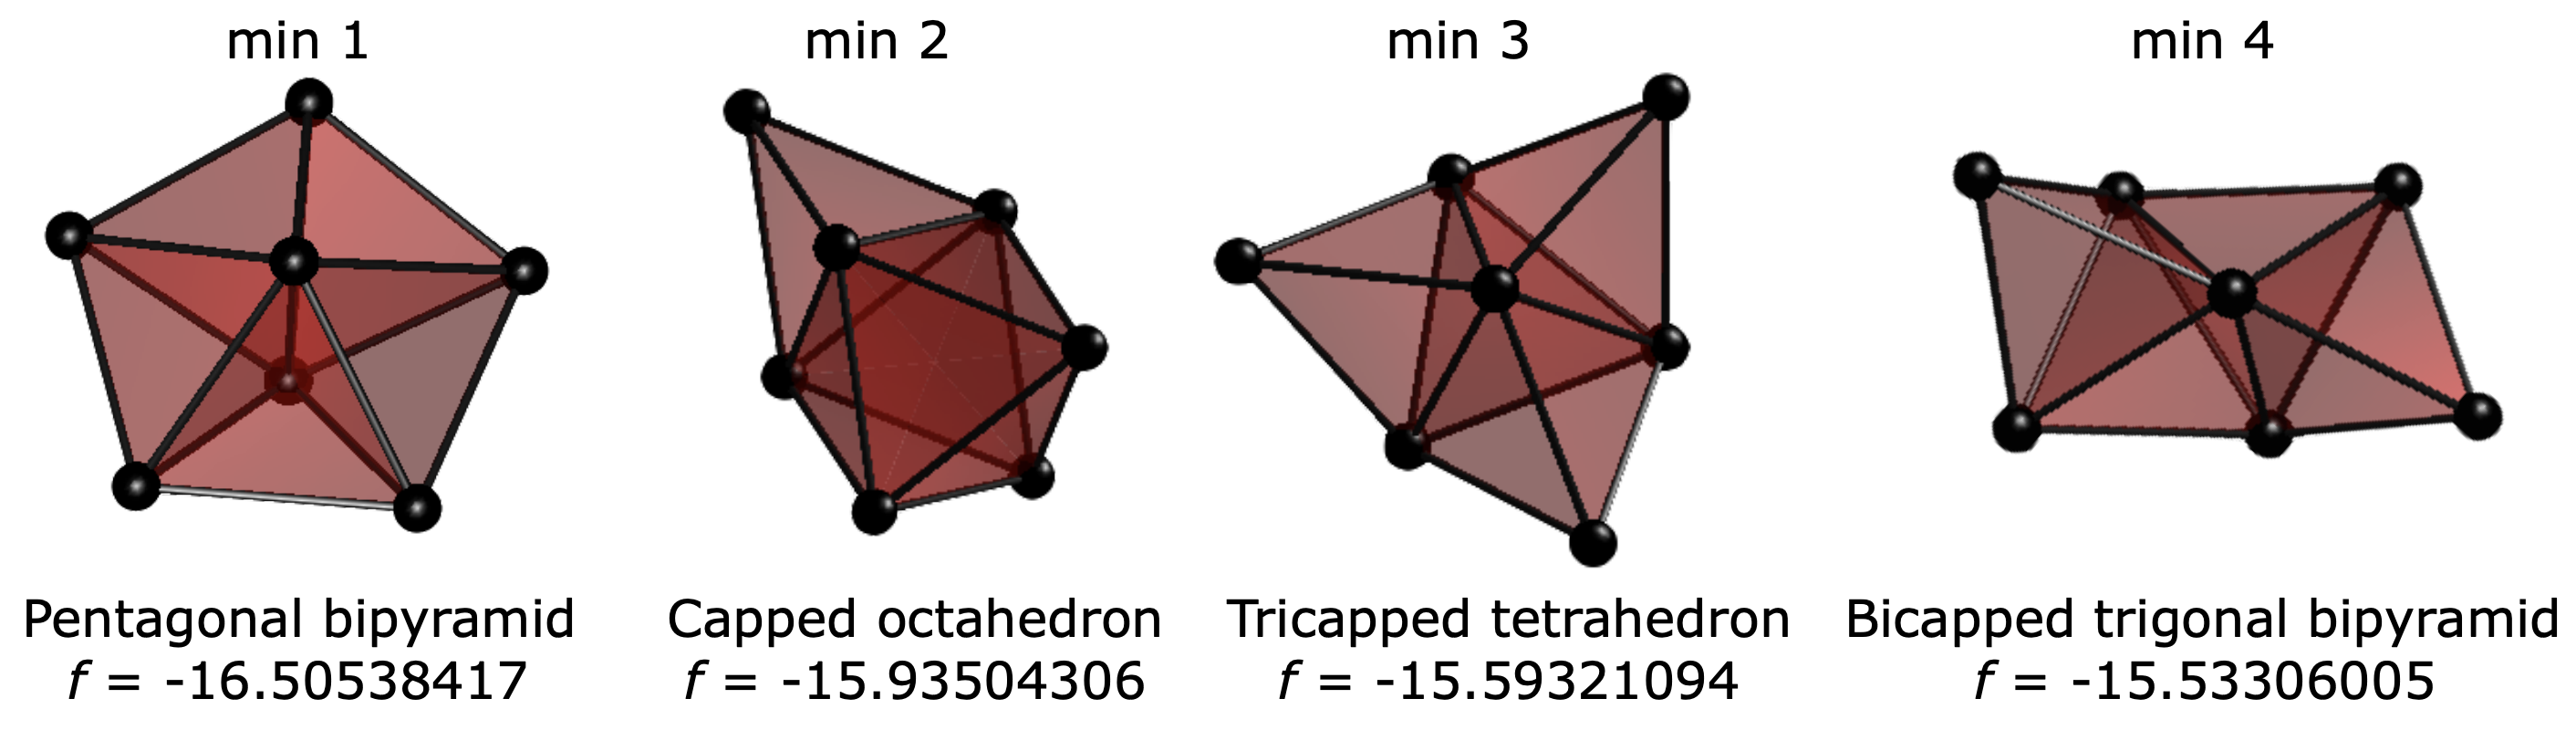
\includegraphics[scale=0.2]{minima.png}
  \end{center}
  Add the BFGS search directions to the provided Matlab or Python codes. It is recommended to reset the matrix $B_k$ in the BFGS method to the identity every $m$th step. Try $m = 5$ and $m = 20$.

  Compare the performance of the three algorithms, the steepest descent, Newton's (already encoded), and BFGS in terms of the number of iterations required to achieve convergence and by plotting the graph of $f$ and $\lVert \nabla f \rVert$ against the iteration number for each test case. Do it for each of the four initial conditions approximating the four local minima and ten random initial conditions.
  \begin{solution}
    TODO
  \end{solution}

  \question (Approx. Problem 3.1 from [NW])
  \begin{enumerate}
    \item Compute the gradient and the Hessian of the Rosenbrock function
    \begin{equation}
      \label{eq:rosenbrock}
      f(x, y) = 100(y - x^2)^2 + (1 - x)^2.
    \end{equation}
    Show that $(1, 1)$ is the only local minimizer, and that the Hessian is positive definite at it.
    \begin{solution}
      TODO
    \end{solution}
    \item Program the steepest descent, Newton's, and BFGS algorithms using the backtracking line search. Use them to minimize the Rosenbrock function (\ref{eq:rosenbrock}). First start with the initial guess $(1.2, 1.2)$ and then with the more difficult one $(-1.2, 1)$. Set the initial step length $\alpha_0 = 1$ and plot the step length $\alpha_k$ versus $k$ for each of the methods.

    Plot the level sets of the Rosenbrock function using the command \texttt{contour} and plot the iterations for each method over it.

    Plot $\lVert (x_k, y_k) - (x^*, y^*) \rVert$ versus $k$ in the logarithmic scale along the $y$-axis for each method. Do you observe a superlinear convergence? Compare the performance of the methods.
    \begin{solution}
      TODO
    \end{solution}
  \end{enumerate}
\end{questions}

\end{document}
